\begin {document}

\chapter{Interpretation der Ergebnisse (VR)}

\section{H\"ohenruder Trimmkurve}

\begin{figure}[h]
	\centering
		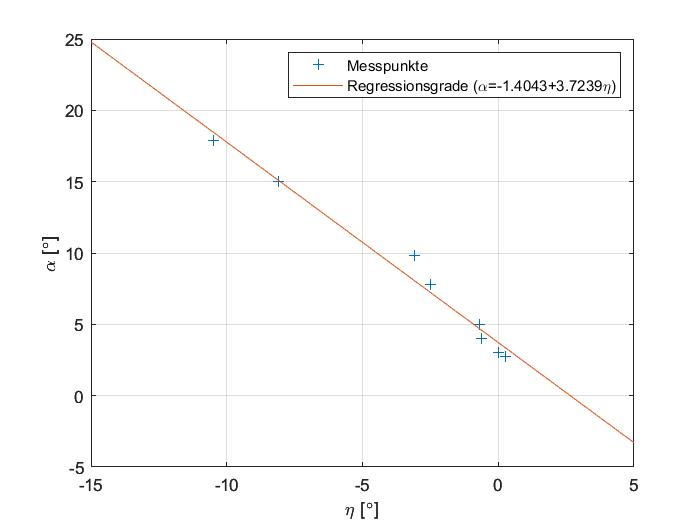
\includegraphics{C:/Users/vrein_000/Documents/git/Labor IFF/Labor-IFF-Flugversuch/Bilder/alpha_eta_plot.jpg}
	\caption{H\"ohenruder-Trimmkurve}
	\label{fig:alpha_eta_plot}
\end{figure}

Aus den aufgezeichneten Daten l\"asst sich ein linearer Zusammenhang zwischen dem Anstellwinkel alpha und dem 
H\"ohenruderausschlag eta feststellen. Mit steigendem H\"ohenruderausschlag sinkt der Anstellwinkel. 
Der Anstellwinkel \alpha beschreibt den Winkel zwischen dem Fluggeschwindigkeitsvektor und der Flugzeugl\"angsachse. Ein positiver Winkel \alpha bedeutet, dass die Flugzeugl\"angsachse positiv gegen\"uber dem Fluggeschwindigkeitsvektor gedreht ist. \\

\begin{figure} [h]
	\begin{minipage} [b]
		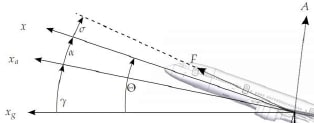
\includegraphics{C:/Users/vrein_000/Documents/git/Labor IFF/Labor-IFF-Flugversuch/Bilder/Anstellwinkel_Definition.jpg}
	\caption{Definition Anstellwinkel}
	\label{alpha_def}
	\end{minipage}

\hspace{0.1\linewidth}
	\begin{minipage} [b]
	\includegraphics{C:/Users/vrein_000/Documents/git/Labor IFF/Labor-IFF-Flugversuch/Bilder/H�henruderausschlag_Definition.jpg}
	\caption{Definition H�henruderausschlag}
	\label{fig:eta_def}
	\end{minipage}
\end{figure}


Der Winkel des H\"ohenruders eta beschreibt die Auslenkung des Ruders gegen\"uber einer Neutrallage. Ein negativer 
H\"ohenruderausschlag bedeutet eine lokale Absenkung des Auftriebs am H\"ohenleitwerk, sodass es zum Absinken des Hecks kommt (Nose-up). In die positive Richtung ausgeschlagen steigt der Auftrieb am H\"ohenleitwerk, sodass sich das Heck hebt (Nosedown). 
Damit decken sich die Messdaten der Do 28 zu Anstellwinkel und H\"ohenruderausschlag mit der Theorie.




\section{Auftriebsbeiwert \"uber Anstellwinkel}

\begin{figure} [t]
	\centering
		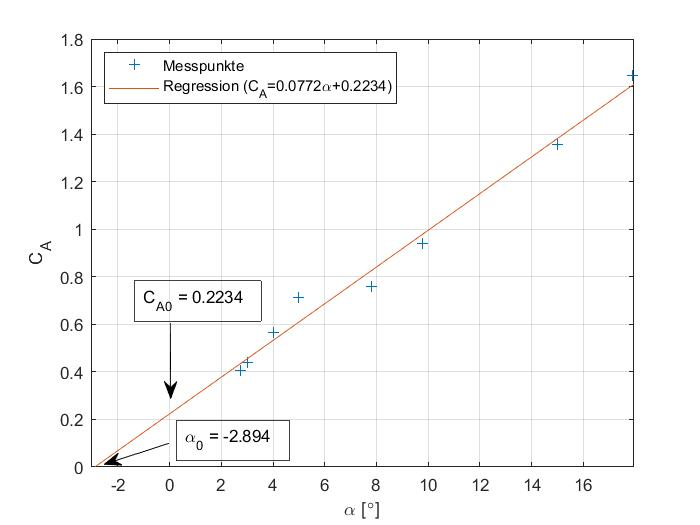
\includegraphics{C:/Users/vrein_000/Documents/git/Labor IFF/Labor-IFF-Flugversuch/Bilder/CA_alpha_plot.jpg}
	\caption{Auftriebsbeiwert �ber Anstellwinkel}
	\label{fig:CA_alpha_plot}
	
\end{figure}


Der Auftriebsbeiwert \(C_a\) steigt linear mit zunehmendem Anstellwinkel alpha. \(C_a0\) bezeichnet den Auftriebsbeiwert bei einem Anstellwinkel von null. \(\alpha_0\) beschreibt den Nullauftriebswinkel, an dem der Auftriebsbeiwert null annimmt, das hei{\ss}t kein Auftrieb mehr generiert wird. Der Auftriebsanstieg \(C_a\alpha\) berechnet sich wie folgt: \\
	\[\(C_a\alpha\)=d\(C_a\)\div \(\alpha\)\] \\
	
Bei der Anstr\"omung eines Tragfl\"ugels wird die Luft umgelenkt und es entsteht eine Druckdifferenz zwischen Tragfl\"ugelober- und Oberseite, was als Voraussetzung f\"ur die Entstehung von Auftrieb ist. Der Anstellwinkel des Fl\"ugels ist dabei der gr\"o{\ss}te Einflussfaktor f\"ur den Auftriebsbeiwert. F\"ur kleine Winkel \alpha mit anliegender Str\"omung gilt daher der lineare Zusammenhang
\[\(C_a\)=\(C_a\alpha\)(\alpha-\(alpha_0\))\] \\

Damit stimmen die Messdaten mit der Theorie \"uberein. Jedoch lassen sich keine Aussagen \"uber den maximalen Auftriebsbeiwert treffen, da die aufgenommenen Anstellwinkel im Bereich der anliegenden Str\"omung liegen und der h\"ochste Auftriebsbeiwert erst kurz vor dem Abrei{\ss}en der Str\"omung erreicht wird. 



\section{Lilienthal-Polare}
\begin{figure} [h]
		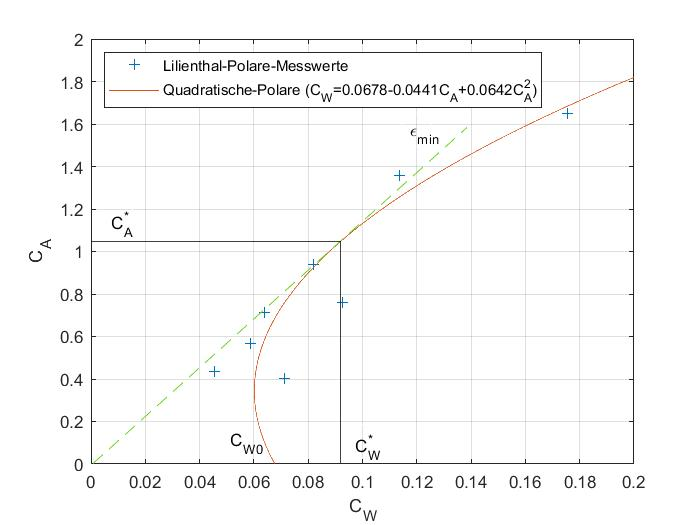
\includegraphics{C:/Users/vrein_000/Documents/git/Labor IFF/Labor-IFF-Flugversuch/Bilder/CA_CW_DO28_NEU.jpg}
	\caption{Do 28}
	\label{fig:CA_CW_DO28}
\end{figure}

Die f�r \(C_A\) und \(C_W\) errechneten Werte werden f�r die Erstellung der Lilienthalpolare gegeneinnder aufgetragen und mit einer quadratischen Regression angen�hert. Daraus ergibt sich f�r den Nullwiderstand \(C_W0\) ein Wert von 0,0503, f�r den Polynomterm erster Ordnung ein Koeffizient von 0,0033 und f�r den zweiten Grades ein Koeffizient von 0,0258. 
Aus der Lillienthal-Polare l�sst sich die minimale reziproke Gleitzahl ermitteln, die die H�hendifferenz beim Sinken des Flugzeugs bei einer bestimmten Flugstrecke beschreibt. Zur Ermittlung der minimalen reziproken Gleitzahl wird eine Tangente durch den Ursprung an die entstandene Polare gelegt. Am Schnittpunkt der Tangente mit der Polaren k�nnen die zugeh�rigen Beiwerte \(C^{*}_A\)=1,39 und  \(C^{*}_W\)=0,105 abgelesen werden, mit denen die reziproke Steigung der Tangente mit

\[ \(\epsilon_min\)=  \(C^{*}_W\) \div \(C^{*}_A\)=0,105 \div 1,39=0,0755\] \\

berechnet werden kann. Der Gleitwinkel \gamma, der die Drehung des Geschwindigkeitsvektor gegen�ber der geod�tischen Horizontalebene in x-Richtung beschreibt, ergibt sich zu

\[\gamma=\arctan(- (\(C^{*}_W\) \div \(C\{*}_)^A\])) = arctan(-(0,105 \div 1,39)) = -4,32~�\]  \\

Aus den bekannten Werten \(C_W0\) und \(C^{*}_A\) l�sst sich der Widerstandsanstieg k wie folgt berechnen: 

\[k= \(C_W0\) \div  \(C^{*} _A\)^{2}=0,0451 \div 1,39^{2}=0,2334 \] \\

 In der Theorie wird an dieser Stelle ein positiver Wert f�r k erwartet, was bedeutet, dass die aus der Regression entnommenen Werte falsch sind. Da nur vier verschiedene Flugzust�nde aufgenommen werden konnten, ist die Regression au�erhalb des Messwertbereichs ungenau. 





\begin{figure}	
	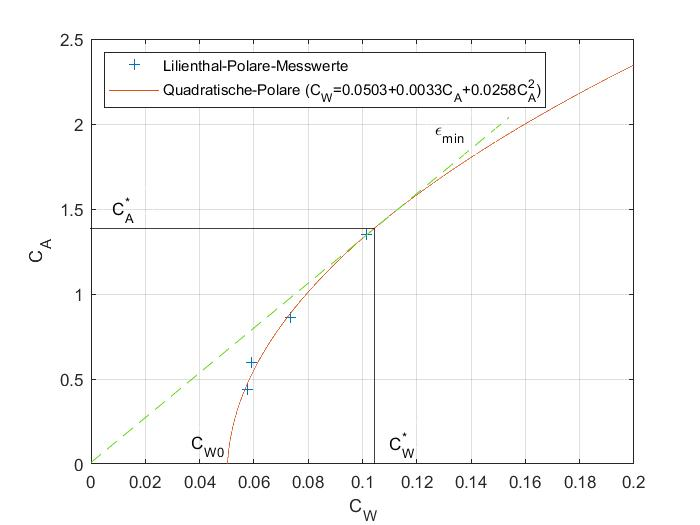
\includegraphics{C:/Users/vrein_000/Documents/git/Labor IFF/Labor-IFF-Flugversuch/Bilder/CA_CW_DO128_NEU.jpg}
	\caption{Do 128}
	\label{fig:CA_CW_DO128_NEU}
\end{figure}




\section{Widerstand \"uber Fluggeschwindigkeit}
tbd

\section{Staudruck \"uber Anstellwinkel}
tbd

\section{Fluggeschwindigkeit \"uber Anstellwinkel}
tbd




\end {document}